\section{Parallelization}





\begin{frame}
\frametitle{Table of contents}

\tableofcontents[currentsection]
\end{frame}





\begin{frame}
\frametitle{Parallelization}

\begin{itemize}
\item Current computer architectures provide multi-core processors
  \begin{itemize}
  \item Supercomputers arrange those on distributed nodes
  \end{itemize}
\item Using all resources efficiently requires parallelization
  \begin{itemize}
  \item Distribution of workload and memory demand
  \end{itemize}
\end{itemize}

\begin{itemize}
\item Our approach: Distribution of domain on several processes
  \begin{itemize}
  \item Each subdomain needs relevant part of the global solution
  \item Requires a layer of so called ghost cells
  \item Involves communication between processors
  \end{itemize}
\end{itemize}

\begin{figure}
\begin{subfigure}{.31\textwidth}
  \centering
  \begin{tikzpicture}
  \LagrangeCell{0}{0}{1}{.08}{1}
  {{"","","",""}};
  \LagrangeCell{1}{0}{1}{.08}{1}
  {{"","","",""}};
  \LagrangeCell{2}{0}{1}{.08}{1}
  {{"","","",""}};
  \end{tikzpicture}
  \caption{Domain to be distributed}
\end{subfigure}
\hspace{-.9ex}\raisebox{.5em}{\(\longrightarrow\)}
\begin{subfigure}{.3\textwidth}
  \centering
  \begin{tikzpicture}
  \fill[color=fzjblue] (0,0) rectangle (1,1);
  \fill[color=fzjblue] (1,0) rectangle (2,1);
  \fill[color=fzjlightblue] (2,0) rectangle (3,1);
  
  \LagrangeCell{0}{0}{1}{.08}{1}
  {{"","","",""}};
  \LagrangeCell{1}{0}{1}{.08}{1}
  {{"","","",""}};
  \LagrangeCell{2}{0}{1}{.08}{1}
  {{"","","",""}};
  \end{tikzpicture}
  \caption{Subdomain for CPU 0}
\end{subfigure}
\begin{subfigure}{.3\textwidth}
  \centering
  \begin{tikzpicture}
  \fill[color=lightgray] (0,0) rectangle (1,1);
  \fill[color=fzjlightblue] (1,0) rectangle (2,1);
  \fill[color=fzjblue] (2,0) rectangle (3,1);
  
  \LagrangeCell{0}{0}{1}{.08}{1}
  {{"","","",""}};
  \LagrangeCell{1}{0}{1}{.08}{1}
  {{"","","",""}};
  \LagrangeCell{2}{0}{1}{.08}{1}
  {{"","","",""}};
  \end{tikzpicture}
  \caption{Subdomain for CPU 1}
\end{subfigure}
%  \vspace{-.3em}
\caption{Illustration of \textcolor{black!10!fzjblue}{\textbf{locally owned}}, \textcolor{black!10!fzjlightblue}{\textbf{ghost}}, and \textcolor{black!10!lightgray}{\textbf{artificial}} cells}
\end{figure}
\end{frame}





\begin{frame}
\frametitle{Parallel hp-adaptive FEM}

\begin{itemize}
\item Combination of hp-adaptive methods with parallelisation
\end{itemize}

\vfill{}

\begin{itemize}
\item The non-trivial parts are:
  \begin{enumerate}
  \item Enumeration of degrees of freedom, independent of number of subdomains
  \item Consignment of contiguous memory chunks for data transfer
  \item Weighted repartitioning for load balancing
  \end{enumerate}
\end{itemize}

\vfill{}

\begin{figure}
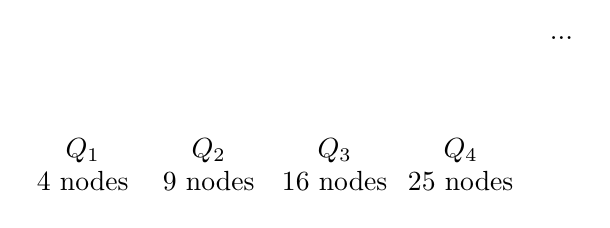
\begin{tikzpicture}[scale=1.6]
\node[align=center] at ( .5,-.5) {$Q_1$ \\  4 nodes};
\node[align=center] at (1.5,-.5) {$Q_2$ \\  9 nodes};
\node[align=center] at (2.5,-.5) {$Q_3$ \\ 16 nodes};
\node[align=center] at (3.5,-.5) {$Q_4$ \\ 25 nodes};

\LagrangeCell{0}{0}{1}{.04}{1}
{{,,,}};
\LagrangeCell{1}{0}{1}{.04}{2}
{{,,,,,,,,}};
\LagrangeCell{2}{0}{1}{.04}{3}
{{,,,,,,,,,,,,,,,}};
\LagrangeCell{3}{0}{1}{.04}{4}
{{,,,,,,,,,,,,,,,,,,,,,,,,,}};

\node at (4.3,.5) {...};
\end{tikzpicture}
\caption{Different finite elements and their number of nodes in 2D}
\end{figure}
\end{frame}





\subsection{Example: Laplace equation}





\begin{frame}
\frametitle{Example: Load balancing}

\begin{figure}
\only<1>{
  \vspace{-.7em}
  \begin{tikzpicture}
  \begin{axis}[
  scale=1,
  xmin=-1,xmax=1,
  ymin=-1,ymax=1,
  unit vector ratio={1 1},
  tick align=outside,
  xlabel=$x$,
  ylabel=$y$,
  colormap/Paired,
  colorbar sampled,
  colorbar style={ylabel={subdomain}, samples=13, ytick={0,1,...,11}},
  colormap access=piecewise const,
  point meta min=-.5,
  point meta max=11.5
  ]
  
  \addplot graphics [
  xmin=-1,xmax=1,
  ymin=-1,ymax=1,
  ] {illustrations/corner-subdomains-legendre-00.pdf};
  \end{axis}
  \end{tikzpicture}
  \vspace{-.7em}
  \caption{Mesh decomposition in cycle 0.
Weights assigned to cells are $\propto n_\text{dofs}^{1.9}$.}
}
\only<2>{
  \vspace{-.7em}
  \begin{tikzpicture}
  \begin{axis}[
  scale=1,
  xmin=-1,xmax=1,
  ymin=-1,ymax=1,
  unit vector ratio={1 1},
  tick align=outside,
  xlabel=$x$,
  ylabel=$y$,
  colormap/Paired,
  colorbar sampled,
  colorbar style={ylabel={subdomain}, samples=13, ytick={0,1,...,11}},
  colormap access=piecewise const,
  point meta min=-.5,
  point meta max=11.5
  ]
  
  \addplot graphics [
  xmin=-1,xmax=1,
  ymin=-1,ymax=1,
  ] {illustrations/corner-subdomains-legendre-01.pdf};
  \end{axis}
  \end{tikzpicture}
  \vspace{-.7em}
  \caption{Mesh decomposition in cycle 1.
Weights assigned to cells are $\propto n_\text{dofs}^{1.9}$.}
}
\only<3>{
  \vspace{-.7em}
  \begin{tikzpicture}
  \begin{axis}[
  scale=1,
  xmin=-1,xmax=1,
  ymin=-1,ymax=1,
  unit vector ratio={1 1},
  tick align=outside,
  xlabel=$x$,
  ylabel=$y$,
  colormap/Paired,
  colorbar sampled,
  colorbar style={ylabel={subdomain}, samples=13, ytick={0,1,...,11}},
  colormap access=piecewise const,
  point meta min=-.5,
  point meta max=11.5
  ]
  
  \addplot graphics [
  xmin=-1,xmax=1,
  ymin=-1,ymax=1,
  ] {illustrations/corner-subdomains-legendre-02.pdf};
  \end{axis}
  \end{tikzpicture}
  \vspace{-.7em}
  \caption{Mesh decomposition in cycle 2.
Weights assigned to cells are $\propto n_\text{dofs}^{1.9}$.}
}
\only<4>{
  \vspace{-.7em}
  \begin{tikzpicture}
  \begin{axis}[
  scale=1,
  xmin=-1,xmax=1,
  ymin=-1,ymax=1,
  unit vector ratio={1 1},
  tick align=outside,
  xlabel=$x$,
  ylabel=$y$,
  colormap/Paired,
  colorbar sampled,
  colorbar style={ylabel={subdomain}, samples=13, ytick={0,1,...,11}},
  colormap access=piecewise const,
  point meta min=-.5,
  point meta max=11.5
  ]
  
  \addplot graphics [
  xmin=-1,xmax=1,
  ymin=-1,ymax=1,
  ] {illustrations/corner-subdomains-legendre-03.pdf};
  \end{axis}
  \end{tikzpicture}
  \vspace{-.7em}
  \caption{Mesh decomposition in cycle 3.
Weights assigned to cells are $\propto n_\text{dofs}^{1.9}$.}
}
\only<5>{
  \vspace{-.7em}
  \begin{tikzpicture}
  \begin{axis}[
  scale=1,
  xmin=-1,xmax=1,
  ymin=-1,ymax=1,
  unit vector ratio={1 1},
  tick align=outside,
  xlabel=$x$,
  ylabel=$y$,
  colormap/Paired,
  colorbar sampled,
  colorbar style={ylabel={subdomain}, samples=13, ytick={0,1,...,11}},
  colormap access=piecewise const,
  point meta min=-.5,
  point meta max=11.5
  ]
  
  \addplot graphics [
  xmin=-1,xmax=1,
  ymin=-1,ymax=1,
  ] {illustrations/corner-subdomains-legendre-04.pdf};
  \end{axis}
  \end{tikzpicture}
  \vspace{-.7em}
  \caption{Mesh decomposition in cycle 4.
Weights assigned to cells are $\propto n_\text{dofs}^{1.9}$.}
}
\only<6>{
  \vspace{-.7em}
  \begin{tikzpicture}
  \begin{axis}[
  scale=1,
  xmin=-1,xmax=1,
  ymin=-1,ymax=1,
  unit vector ratio={1 1},
  tick align=outside,
  xlabel=$x$,
  ylabel=$y$,
  colormap/Paired,
  colorbar sampled,
  colorbar style={ylabel={subdomain}, samples=13, ytick={0,1,...,11}},
  colormap access=piecewise const,
  point meta min=-.5,
  point meta max=11.5
  ]
  
  \addplot graphics [
  xmin=-1,xmax=1,
  ymin=-1,ymax=1,
  ] {illustrations/corner-subdomains-legendre-05.pdf};
  \end{axis}
  \end{tikzpicture}
  \vspace{-.7em}
  \caption{Mesh decomposition in cycle 5.
Weights assigned to cells are $\propto n_\text{dofs}^{1.9}$.}
}
\end{figure}
\end{frame}




\begin{frame}
\frametitle{Example: Strong scaling}

\vspace{-1em}

\begin{figure}
\begin{tikzpicture}
\begin{loglogaxis}[
scale=0.9,
xlabel={Number of MPI processes},
ylabel={Wall time [seconds]},
grid=major,
legend cell align=left,
legend pos=outer north east,
legend style={font=\tiny}
]
% data
\addplot table [y=solve, x=ncpus, col sep=comma] {data/strong/strong-nrefs12.csv};
\addlegendentry{linear solver and preconditioner};

\addplot table [y=setup, x=ncpus, col sep=comma] {data/strong/strong-nrefs12.csv};
\addlegendentry{setup data structures};

\addplot table [y=assembly, x=ncpus, col sep=comma] {data/strong/strong-nrefs12.csv};
\addlegendentry{assemble linear system};

\addplot table [y=compute errors, x=ncpus, col sep=comma] {data/strong/strong-nrefs12.csv};
\addlegendentry{estimate error};

\addplot table [y=calculate indicators, x=ncpus, col sep=comma] {data/strong/strong-nrefs12.csv};
\addlegendentry{estimate smoothness};

\addplot table [y=refine, x=ncpus, col sep=comma] {data/strong/strong-nrefs12.csv};
\addlegendentry{coarsen and refine};

% optimal line
\addplot[very thick, samples=2, domain=768:49152] {10^(5)*x^(-1)};
\addlegendentry{optimal convergence};

% auxiliary lines
\begin{scope}
\draw[green, very thick] ({axis cs:9692.57276,0}|-{rel axis cs:0,1}) -- ({axis cs:9692.57276,0}|-{rel axis cs:0,0});
\end{scope}
\addlegendimage{color=green};
\addlegendentry{$10^5$ DoFs per process};
\end{loglogaxis}
\end{tikzpicture}
\caption{Strong scaling for fixed problem size of $\sim$ 970 million degrees of freedom}
\end{figure}
\end{frame}